\documentclass{article}
\usepackage{tikz}
\usetikzlibrary{patterns}
\begin{document}

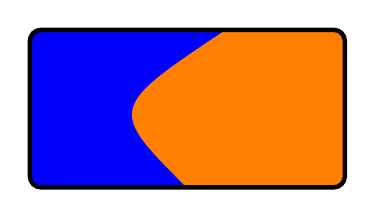
\begin{tikzpicture}
\draw[fill, blue] 
    {[rounded corners] (0, 0) -- (0,   2)} % ← a group
                              -- (2.5, 2)
        .. controls (1, 1) and (1, 1) .. (2, 0)
    [rounded corners] -- cycle;            % ← rest of the path

\draw[fill, orange] 
     [rounded corners] (4, 0) -- (4,   2)
     [sharp corners]          -- (2.5, 2)  % ← switch back
        .. controls (1, 1) and (1, 1) .. (2, 0)
     [rounded corners] -- cycle;           % ← and forth

\draw[ultra thick,rounded corners]
    (0,0) rectangle (4,2);
\end{tikzpicture}

\tikz
\draw[ultra thick,rounded corners]
    (0,0) rectangle (4,2)[path picture={
        \draw[fill, blue] (0, 0) |- (2.5, 2) 
                .. controls (1, 1) and (1, 1) .. (2, 0)
          -- cycle;
        \draw[fill, orange] (4, 0) |- (2.5, 2) 
                .. controls (1, 1) and (1, 1) .. (2, 0)
              -- cycle;
    }];
\end{document}